\documentclass{article} % For LaTeX2e
\usepackage{nips14submit_e,times}
\usepackage{amsmath}
\usepackage{amsthm}
\usepackage{amssymb}
\usepackage{mathtools}
\usepackage{hyperref}
\usepackage{url}
\usepackage{algorithm}
\usepackage[noend]{algpseudocode}
%\documentstyle[nips14submit_09,times,art10]{article} % For LaTeX 2.09

\usepackage{graphicx}
\usepackage{caption}
\usepackage{subcaption}

\def\eQb#1\eQe{\begin{eqnarray*}#1\end{eqnarray*}}
\def\eQnb#1\eQne{\begin{eqnarray}#1\end{eqnarray}}
\providecommand{\e}[1]{\ensuremath{\times 10^{#1}}}
\providecommand{\pb}[0]{\pagebreak}
\DeclarePairedDelimiter\ceil{\lceil}{\rceil}
\DeclarePairedDelimiter\floor{\lfloor}{\rfloor}

\newcommand{\E}{\mathrm{E}}
\newcommand{\Var}{\mathrm{Var}}
\newcommand{\Cov}{\mathrm{Cov}}

\def\Qb#1\Qe{\begin{question}#1\end{question}}
\def\Sb#1\Se{\begin{solution}#1\end{solution}}

\newenvironment{claim}[1]{\par\noindent\underline{Claim:}\space#1}{}
\newtheoremstyle{quest}{\topsep}{\topsep}{}{}{\bfseries}{}{ }{\thmname{#1}\thmnote{ #3}.}
\theoremstyle{quest}
\newtheorem*{definition}{Definition}
\newtheorem*{theorem}{Theorem}
\newtheorem*{lemma}{Lemma}
\newtheorem*{question}{Question}
\newtheorem*{preposition}{Preposition}
\newtheorem*{exercise}{Exercise}
\newtheorem*{challengeproblem}{Challenge Problem}
\newtheorem*{solution}{Solution}
\newtheorem*{remark}{Remark}
\usepackage{verbatimbox}
\usepackage{listings}
\usepackage{mathrsfs}
\title{ProbLimI: \\
Pset I}


\author{
Youngduck Choi \\
CIMS \\
New York University\\
\texttt{yc1104@nyu.edu} \\
}


% The \author macro works with any number of authors. There are two commands
% used to separate the names and addresses of multiple authors: \And and \AND.
%
% Using \And between authors leaves it to \LaTeX{} to determine where to break
% the lines. Using \AND forces a linebreak at that point. So, if \LaTeX{}
% puts 3 of 4 authors names on the first line, and the last on the second
% line, try using \AND instead of \And before the third author name.

\newcommand{\fix}{\marginpar{FIX}}
\newcommand{\new}{\marginpar{NEW}}

\nipsfinalcopy % Uncomment for camera-ready version

\begin{document}


\maketitle

\begin{abstract}
This work contains solutions to the exercises of the problem set I.
\end{abstract}

\bigskip

\begin{question}[1]
\hfill
\begin{figure}[h!]
  \centering
    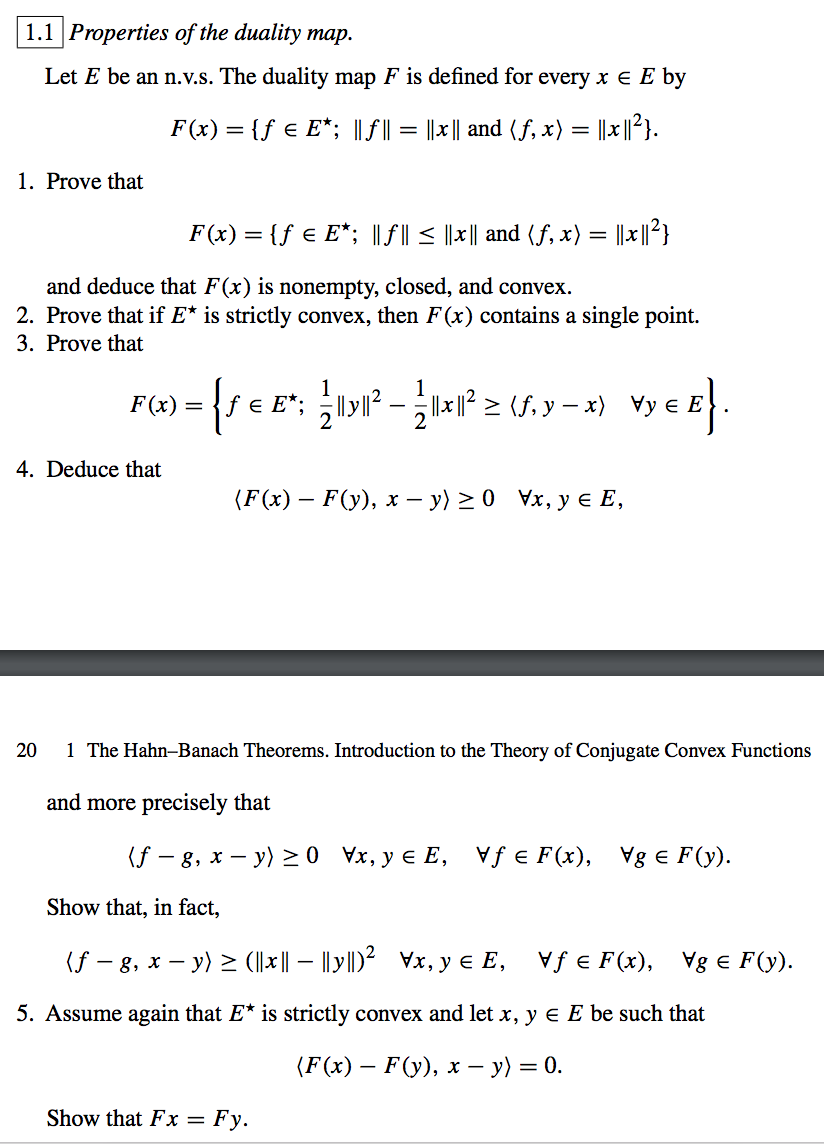
\includegraphics[width=0.7\textwidth]{funcA-1-1.png}
\end{figure}
\end{question}
\begin{solution} \hfill \\
\textbf{(1)} The first set equality follows as 
\eQb
f \in E^* \>\>\> \text{ and} \>\>\> < f, x >  \> = ||x||^2 \implies ||f|| \geq ||x||,
\eQe
because otherwise 
\eQb
|<f , x>| &=& ||x||^2 > ||f|||x||,
\eQe
which is absurd. Now, by Corollary 1.3, it follows that $F(x)$ is non-empty.

\smallskip 
 
We show that $F(x)$ is convex. Let $f,g \in F(x)$ and $t \in [0,1]$. Then,
it follows that
\eQb
< t f + (1-t)g, x> &=& t<f,x> + (1-t)<g,x> = ||x||^2 
\eQe 
and
\eQb
||t f + (1-t)g|| &\leq& t||f|| + (1-t)||g|| \leq ||x||,
\eQe
so $tf + (1-t)g \in F(x)$ and $F(x)$ is convex. 

\smallskip

We show that $F(x)$ is closed. Let $f \in E^*$ such that there exists $\{f_n\} \subset
F(x)$ with $f_n \to f$. As convergence in dual norm implies pointwise convergence,
we have
\eQb
||x||^2 = <f_n, x> \to <f,x> \>\> \text{ and } \>\> <f,x> = ||x||^2. 
\eQe
Also, as $||f_n - f|| \to 0$, and by reverse-triangle inequality, we have
\eQb
||f_n|| \to ||f|| \>\> &\text{and}& \>\> ||f|| \leq ||x||, 
\eQe 
which shows that $f \in F(x)$, and consequently that $F(x)$ is closed.

\bigskip

\textbf{(2)} 

\end{solution}

\newpage


\begin{question}[2]
\hfill
\begin{figure}[h!]
  \centering
    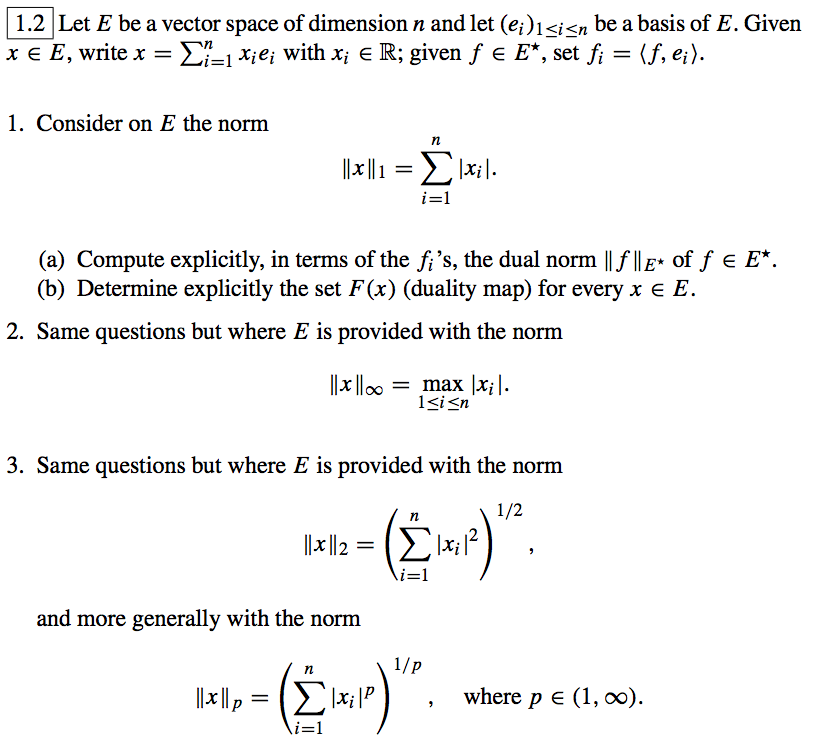
\includegraphics[width=0.7\textwidth]{funcA-1-2.png}
\end{figure}
\end{question}
\begin{solution} \hfill \\
\end{solution}
\bigskip

\begin{question}[3]
\hfill
\begin{figure}[h!]
  \centering
    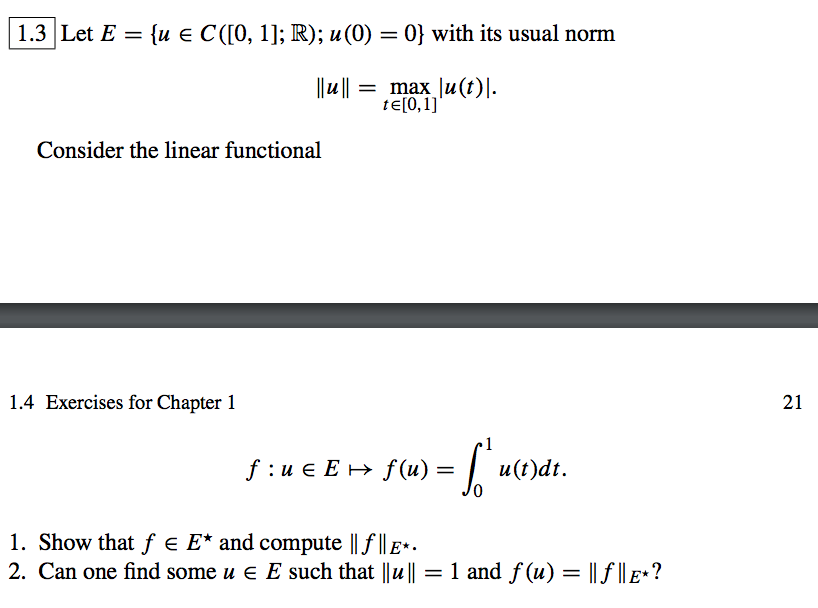
\includegraphics[width=0.7\textwidth]{funcA-1-3.png}
\end{figure}
\end{question}
\begin{solution} \hfill \\
\end{solution}
\bigskip

\begin{question}[4]
\hfill
\begin{figure}[h!]
  \centering
    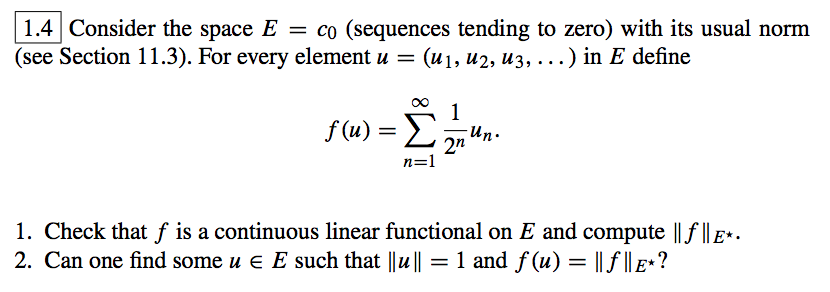
\includegraphics[width=0.7\textwidth]{funcA-1-4.png}
\end{figure}
\end{question}
\begin{solution} \hfill \\

\textbf{(2)} Suppose for sake of contradiction that there exists $u \in c_0$, such that
\eQb
||u|| = 1 \>\> \text{and} \>\> f(u) = 1.
\eQe
Choose $N > 1$ such that 
\eQb
n \geq N \>\> &\implies& \>\>  u_n < \dfrac{1}{2}.
\eQe
Then,
\eQb
f(u) &<& \sum_{n=1}^{N-1} \dfrac{1}{2^n} u_n  + \dfrac{1}{2} 
\sum_{n=N}^{\infty}\dfrac{1}{2^n} = 
\sum_{n=1}^{N-1} \dfrac{1}{2^n} u_n + \dfrac{1}{2^{N+1}}. \\ 
\eQe

\end{solution}

\end{document}

